\documentclass{report}%[11pt,a4paper]


\usepackage[a4paper, total={6in, 8in}]{geometry}
%\usepackage{float}
\usepackage{enumerate}
\usepackage{graphicx}
\graphicspath{ {images/} }
%\usepackage{url}
\usepackage{multirow}
\usepackage{algorithm}
\usepackage{algorithmicx}
\usepackage{algpseudocode}
\usepackage{amsmath}
\usepackage{amssymb}
%\usepackage{makeidx}
%\makeindex

\begin{document}

\title{Literature Review of Optimisation Techniques to the Graph Colouring Problem}
\author{Scott Whitemore \& Brendon Veronese}

\floatstyle{boxed} 
\restylefloat{figure}

\maketitle
\begin{abstract}
A review of papers concerning the current state-of-the-art for solving the GCP is presented. Algorithms from these papers are implemented and compared, results are shown in an unbiased way. 
\end{abstract}

\chapter{Literature Review}

\section{Introduction}

The graph coloring problem has widespread applications in areas such as scheduling and timetabling.

Bondy and Murty describe graph coloring as follows:
\begin{quotation}
A $k-vertex colouring$ of $G$ is an assignment of $k$ colours, $1,2,\ldots,k$, to the vertices of $G$; the colouring is \emph{proper} if no two distinct adjacent vertices have the same colour. Thus a proper $k$-vertex colouring of a loopless graph $G$ is a partition $(V_1,V_2,\ldots,V_k)$ of $V$ into $k$ (possibly empty) independent sets. $G$ is $k-vertex-colourable$ if $G$ has a proper $k$-vertex colouring. It will be convenient to refer to a `proper $k$-vertex colouring as a $k-colouring$'.
The \emph{chromatic number}, $\chi(G)$, of $G$ is the minimum $k$ for which $G$ is $k$-colourable; if $\chi(G)=k$, $G$ is said to be $k-chromatic$
\end{quotation}

The Graph Coloring Problem (GCP) is the task of trying to find the value for $\chi(G)$ for some given $G$, however, this is an NP-Hard problem of at least $O(N)$ complexity and so finding a $k$ that is guaranteed to be $\chi(G)$ is often ($N>$ single digits) impossible. As such we hope to be able to develop heuristic algorithms that are able to find near-optimal colorings ($k \rightarrow \chi(G)$) quickly (seconds/minutes/hours depending on the size and complexity of the graph).

This work is laid out as follows:
In chapter 1 we will introduce four different methods for solving the GCP that have been proposed by other authors: Simulated Annealing, Gravitational Swarm Intelligence, Genetic Algorithm and Flower Pollination Algorithm. The papers that describe these algorithms, as well as the algorithms themselves, vary in quality and we will be commenting on particularly bad or confusing aspects as they crop up.
We attempted to implement the latter three methods in Java going off of just what was provided in the papers, to mixed success. A write up of these attempts, as well as some pseudocode, is presented in chapter 2.
Finally, chapter 3 has the results of applying the three algorithms to some of the DIMACS benchmark graphs.


\section{Johnson - Simulated Annealing}

Johnson et al.'s three part series on Simulated Annealing published in 1991 is perhaps the seminal work on the subject. The second part of the series covers the well studied yet never satisfactorily solved \emph{Graph Coloring Problem}. You didn't see that one coming did you?\\

The paper begins by introducing introducing the context, including what the GCP is, and presenting a general simulated annealing algorithm.

So what is simulated annealing? Simulated annealing is an adjustment to local optimisation that has the ability to escape local optima (to a point). By using a temperature parameter that reduces as the algorithm progresses to govern when an uphill move can be made, simulated annealing is able to move around the solution space easily at early iterations but becomes locked in at later iterations.

In order to approach the GCP from an optimisation stand point three components of the optimisation scheme have to be established: a neighbourhood graph that describes the solution space, a way to move through the solution space, and an initial solution.

Three types of neighbourhoods and movement strategies are proposed, leading to three different SA algorithms for solving the GCP. All algorithms use some sort of randomised initial solution suitable for their particular implementation.

\subsection{Penalty Function approach}

\begin{itemize}
	\item A solution will be \emph{any} partition of $V$ into nonempty disjoint sets $C_1,C_2,\ldots,C_k$, whether the $C_i$ are legal color classes or not.
	\item Two solutions are neighbours if one can be transformed to the other by moving a vertex from one color class to another.
	\item To generate a random neighbour by randomly picking a nonempty color class $C_{OLD}$, a vertex $v \in C_{OLD}$, and then an integer $i,\,1 \leq i \leq k+1$. The neighbour is obtained by moving $v$ to $C_i$. If $i = k+1$ then $v$ is moved to a new, previously empty class.
	\item Note that this biases the choice of $v$ towards vertices in smaller color classes.
	\end{itemize}


\begin{itemize}
	\item Adopts the general philosophy of RLF, which constructs its colorings with the aid of a subroutine for generating large independent sets.
	\item Cost function has two components, the first favours large color classes, the second favours independent sets.
	\item Let $\Pi = (C_1,\ldots,C_k)$ be a solution and $E_i, \, 1 \leq i \leq k$ be the set of edges from $E$ both of whose endpoints are in $C_i$, i.e., the set of \emph{bad} edges in $C_i$.
	\item Cost Function
		\begin{equation*}
		\centering
		cost(\Pi) = - \displaystyle \sum_{i=1}^{k} |C_i|^2 + \sum_{i=1}^{k} 2|C_i| \dot |E_i|
		\end{equation*}
	\end{itemize}

\subsection{Kempe Chain approach}

\begin{itemize}
\item Solutions are now restricted to be partitions $C_1,C_2,\ldots,C_k$ that are legal colorings.
\item Cost function simplifies to
\begin{equation*}
cost(\Pi) = - \displaystyle \sum_{i=1}^{k} |C_i|^2.
\end{equation*}
\item Moves through the solution space are based on \emph{Kempe Chains}
\end{itemize}

\begin{itemize}
	\item Suppose that $C$ and $D$ are disjoint independent sets in a graph $G$.
	\item A Kempe chain for $C$ and $D$ is any connected component in the subgraph of $G$ induced by $C \cup D$.
	\item Let $X \Delta Y$ denote the symmetric difference $(X-Y)\cup(Y-X)$.
	\item Let $H$ be a Kempe chain of $C$ and $D$, then $C \Delta H$ and $D \Delta H$ are themselves disjoint independent sets whose union is $C \cup D$.
\end{itemize}

\begin{itemize}
	\item Randomly choose a nonempty color class $C$ and a vertex $v \in C$.
	\item Randomly choose a nonempty color class $D$ other than $C$
	\item Let $H$ be the \emph{Kempe chain} for $C$ and $D$ that contains $v$.
	\item Repeat until one obtains $C , D , v$ and $H$ s.t. $H \neq C \cup D$
	\item The next partition is obtained by replacing $C$ by $C \Delta H$ and $D$ by $D \Delta H$ 
	\end{itemize}

\subsection{Fixed-K approach}
	\begin{itemize}
	\item Takes a different approach to the previous methods. As the name suggests, this algorithm runs for some fixed $k$.
	\item Solutions are any partitioning of $V$ into $k$ color classes.
	\item Attempts to minimise the number of \emph{bad} edges.
	\item A partition $\Pi_2$ is a neighbour of a partition $\Pi_1$ if the two partitions differ only as to the position of a single vertex $v$ and $v$ is an endpoint of a bad edge in $\Pi_1$.
	\item A legal coloring has no neighbours since if a legal coloring is found the algorithm stops.
	\end{itemize}

\subsection{Testing}

In order to form a comparison to the current methodologies of the time, three Successive Augmentation algorithms are also run: DSATUR, RLF and XRLF (an extension of the former).
All algorithms are run on random graphs of various sizes and edge probabilities, some ``cooked'' graphs that have chromatic numbers approximately half the equivalent random graph, and some geometric graphs that have certain properties as well as their complements.

\subsection{Author's Conclusions}

\begin{itemize}
	\item Experimental results did not allow the authors to identify a best graph coloring heuristic. Rather, they feel that their results reinforce the notion that there is no best heuristic.
	\item In general Kempe chain annealing starts to take over fixed-K annealing as density increases. This makes sense given their neighbourhood structure.
	\item Penalty function annealing, Kempe chain annealing and RLF are biased towards favouring unbalanced colorings, i.e. better a large and a small sized class than two equally sized classes. Fixed-K on the other hand is neutral, potentially giving it an advantage on graphs whose good colorings are balanced.
	\end{itemize}


\subsection{Wrap-up}

Johnson et al. 1991 is a highly regarded and often referenced mainstay in the field of optimisation for good reason. The paper is well written, describes the methods in good detail and reports on extensive experimentation. 
On a personal note, I was very disappointed that the manuscript by Shapiro and Morgenstern that Johnson et al. cites for their Kempe Chain implementation is not available online and in fact only exists as a physical copy in three locaitons in the world: Centrum Wiskunde en Informatica - Amsterdam, NL 1098 XG Netherlands; University of New Mexico-Main Campus - Albuquerque, NM 87131 United States; and Stanford University Libraries - Stanford, CA 94305 United States.

%\subsection{Critique}
%I wish I'd been able to implement Kemp chain annealing, it's such a cool idea and was shown to be able to find colorings on huge graphs that none of the others could even come close to.\\
%By any modern standard these algorithms are slow - more modern optimisation techniques absolutely destroy them. SA in general is actually pretty bad, even the modern and highly confusing quantum tunnelling SA algorithm is shown in to be beaten easily by the gravitational swarm. And yet oddly, none of them can hope to compete with Wendy's random buckets... such a strange state of affairs.

\section{Gravitational Swarm Intelligence}
\paragraph*{} The natural inspiration of this algorithm does not come from living beings, such as ants or bees, but from the basic physical law of gravitational attraction between objects. We construct a world that agents navigate through, attracted by the gravitational pull of specific objects, the color goals, such that they may suffer specific repulsion forces, activated by the friend-or-foe nature of the relation between agents induced by the adjacency relation in the underlying graph.
\paragraph*{} \textbf{Initial definition}: Let $G = (V,E)$ be a graph defined on a set of nodes $V = \lbrace v_1,\ldots,v_N \rbrace$ and edges $E \subseteq V \times V$. We define a group of GS-GC agents $B = \lbrace b_1, b_2, \ldots , b_N \rbrace$ each corresponding to a graph node. Each agent navigates inside a square planar toric world according to a speed vector $\overrightarrow{v_i}$. At any moment in time we know the position attribute of each agent $p_i(t) = (x_i,y_i)$ where $x_i$ and $y_i$ are the Cartesian coordinates in the space. When $t = 0$ we have the initial position of the agents $p_i(0) = (x_0, y_0)$. Suppose that we want to color the graph with $K$ colors, denoting $C = \lbrace 1, 2, \ldots , K \rbrace$ the set of colors, where K must not be lower than the chromatic number of the graph for the GS-GC to converge. We assign to these colors, $K$ fixed points in space, the color goals $CG = \lbrace g_1 , \ldots , g_K \rbrace$, endowed with a gravitational attraction resulting in a  velocity component $\overrightarrow{v_{gc}}$ affecting the agents. The attraction force decreases with the distance, but affects all the agents in the space.
\paragraph*{} The problem collapses into the minimisation of a cost function:
\[ min | \lbrace b_i \textbf{ s.t. } b_i \in \lbrace g_1, \ldots g_N \rbrace \rbrace | \]
We denote the set of agents whose position is in the region of the space near enough to a color neighbourhood of the color as:

\begin{equation}
\mathcal{N} \left( g_k \right) = \lbrace b_i \textbf{ s.t. } \Vert p_i - g_k \Vert < nearenough \rbrace
\end{equation}

We denote the fact that the node has been assigned to the corresponding color assigning value to a the agent color attribute

\begin{equation}
b_i \in \mathcal{N}\left( g_k \right) \Rightarrow c_i = k
\end{equation}

The initial value of the agent color attribute $c_i$ is zero or null. Inside the spatial neighbourhood of a color goal there is no further gravitational attraction. However, there may be a repulsion force between agents that are connected with an edge in the graph G. This repulsion is only effective for agents inside the same color goal neighbourhood. To model this effect, we define function repulsion which has value 1 if a pair of GS-GC agents have an edge between them, and 0 otherwise. The repulsive forces experimented by agent $b_i$ from the agents in the color goal $g_k$ are computed as follows:

\begin{equation}
R \left( b_i, g_k \right) = \sum\limits_{\mathcal{N}\left( g_k \right)} repulsion \left( b_i, b_j \right)
\end{equation}

The cost function defined on the global system spatial configuration is:

\begin{equation}
f \left( B, CG \right) = | \lbrace b_i \textbf{ s.t. } c_i \in C \& R \left(b_i, g_{c_i} \right) = 0 \rbrace |
\end{equation}

This cost function is the number of graph nodes which have a color assigned and no conflict inside the color goal. The agents outside the neighbourhood of any color goal can't be evaluated, so it can be a part of the solution of the problem. The dimension of the world and the definition of the $nearenough$ threshold allows controlling the speed of convergence of the algorithm. If the world is big and the $nearenough$ variable is small then the algorithm converges slowly but monotonically to the solution, if the world is small and the $nearenough$ variable is big the algorithm is faster but convergence is jumpy because the algorithm falls in local minima and needs transitory energy increases to escape them. The reason of this behaviour is that the world is not normalized and the magnitude of the velocity vector can be larger than the radius of the color goal's spatial influence and this means an agent could potentially cross a goal without being captured by it.
\paragraph*{} Each color goal has an attraction well spanning the entire space, therefore the gravitational analogy. But in our approach the magnitude of the attraction drops proportionally with the Euclidean distance $d$ between the goal and the GS-GC agent, but it never disappears. If $\Vert d \Vert < nearenough$ then we make $d = 0$, and the agent's velocity becomes 0, stopping it.

We now present a more formal definition of the algorithm.
\paragraph*{} \textbf{Definition}: A Gravitational Swarm (GS) is a collection of particles $P = \lbrace p_1, \ldots , p_L \rbrace$ moving in an space $S$ subjected to attraction and repulsion forces. Attraction correspond to long range gravitational interactions. Repulsions correspond to short range electrical interactions. Particle attributes are: spatial localization $s_i \in S$, mass $m_i \in \mathbb{R}$, charge $\mu_i \in \mathbb{R}$, set of repelled particles $r_i \subseteq P$. The motion of the particle in the space is governed by equation:
\begin{equation}
s_i \left( t \right) = -m_i \left( t \right) A_i \left( t \right) + \mu_i \left( t \right) R_i \left( t \right) + \eta \left( t \right)
\end{equation}
where $A_i(t)$ and $R_i(t)$ are the result of the attractive and repulsive forces, and $\eta(t)$ is a random (small) noise term. The attractive motion term is of the form:
\begin{equation}
A_i(t) = \sum \limits_{p_j \in P - r_i} m_j(t)(s_i - s_j) \delta_{ij}^A
\end{equation}
where
\begin{equation}
\delta_{ij}^A = \begin{cases} 
\Vert s_i - s_j \Vert ^{-2} & \Vert s_i - s_j \Vert ^2 > \theta^A \\
0 & \Vert s_i - s_j \Vert ^2 \leq \theta^A 
\end{cases}
\end{equation}
The repulsive term is of the form
\begin{equation}
R_i(t) = \sum \limits_{p_j \in r_i} \mu_j(t)(s_i - s-j) \delta_{ij}^R
\end{equation}
where
\begin{equation}
\delta_{ij}^R = \begin{cases} 
\Vert s_i - s_j \Vert ^{-2} & \Vert s_i - s_j \Vert ^2 \leq \theta^R \\
0 & \Vert s_i - s_j \Vert ^2 > \theta^R 
\end{cases}
\end{equation}
The two delta functions have different roles in the definition of the GS. The attractive $\delta^A$ corresponds to the inverse of the distance and is the strength of attraction. To avoid singular values when two particles are close to zero distance we set a threshold $\theta^A$ which determines the region around the particles where the motion due to attraction forces disappear. The repulsive $\delta^R$ defines for each $ij$, the maximum extension of the repulsive forces, which are short range forces. The threshold $\theta^R$ determines the region around the particles where the repulsive forces are active.

A vertex particle of a GS-GC reaches zero velocity if and only if it is at distance below $\theta^A$ of a color particle and no repulsive particle is in $\theta^R$ range.

A global state of the GS-GC is stationary if and only if all vertex particles are placed in the neighbourhood of some color particle without any repulsive particles located at the same color particle neighbourhood.
If the graph's chromatic number $M^\star$ is smaller than or equal to the number of color particles $M^\star \leq M$, there will be a non-empty set of stationary states of the GS-GC.

Any stationary state of the GS-GC corresponds to a graph colouring.
If the graph's chromatic number is greater than the number of color particles, there are no stationary states in the GS-GC.

These conditions mean that it is always possible to (given enough time) find the chromatic number for a graph. The algorithm to do this is outlined in the following sections.

\section{Genetic Algorithm}
\subsection{Introduction}
The genetic algorithm presented in this review is taken from this paper \cite{bib:GeneticAlg}. The paper presents a hybrid technique that applies a genetic algorithm followed by wisdom of crowds voting. The algorithm uses a variety of parent selection, child production and mutation steps. The methods of parent selection, child production and mutation vary according to the state of the fitness of the overall system. This results in an algorithm that is resistant to capture by local optima and allows for the solution space to 'jitter' around before falling upon a global solution. 

\subsection{Algorithm Discussion}
The algorithm is presented in further detail in the Implementations section. The following discussion focuses on algorithm design and fine tuning for the GCP. The algorithm makes careful note that local optima are a concern to this algorithm, and the danger posed to any GCP solving heuristic algorithm is falling into a local optima and not being able to recover. The algorithm uses several approaches to avoid local optima and to that end, a number of different factors considered. 

The crossover function, the method that produces a new chromosome from two previously existing chromosomes is the result of a tournament between parents, where 4 chromosomes are chosen at random and the best for the first pair becomes the first parent, and the best of the second pair becomes the second parent. The crossover function takes the chromosomes of the parents and cuts them both at the same point. The new chromosome is the first part of the first parent's chromosome with the second part of the second parents chromosome appended to the end. This results in a new chromosome of the same length as the original parents chromosomes, and a potentially vastly different 'bad edge' count. This new chromosome can then be subjected to mutation (at some rate, given to be 0.7 here). This mutation method examines each vertex in the chromosome and tries to improve it if it is part of a 'bad edge'. 

This process is shown to be very efficient at improving the solution space. It falls prone to the problem of local optima though, so an alternative parent selection and mutation method are employed. These new methods simply take the best solution and mutate it. The mutation allows the solution to become worse, instead of simply trying to improve the solution, each bad edge is allowed to become any colour. This results in the best solution having the possibility of improving, but most likely actually becoming worse. This is not a bad thing though, as the solution space is shown to improve over time. 

If no valid solution to the colouring is found after a set number of generations (given to be 20,000 in this paper), then a wisdom of crowds approach is implemented, where the best portion (given to be half) of the chromosomes vote to create a new chromosome. This aggregated chromosome is checked to see if it contains a solution to the graph, if not, it becomes the first chromosome is the next round of generations, and all other chromosomes are discarded. 

\subsection{Observations}
This algorithm can become very stagnated when the best solution is very close to an optimal solution. To improve this part of the algorithm, the algorithm implementation was changed to instead choose the best parent and a random chromosome on some chance. 
\section{Flower Pollination}

%Refs

% @incollection{yang2012flower,
%   title={Flower pollination algorithm for global optimization},
%   author={Yang, Xin-She},
%   booktitle={Unconventional computation and natural computation},
%   pages={240--249},
%   year={2012},
%   publisher={Springer}
% }
% @INPROCEEDINGS{7175923, 
% author={Bensouyad, M. and Saidouni, D.}, 
% booktitle={Cybernetics (CYBCONF), 2015 IEEE 2nd International Conference on}, 
% title={A discrete flower pollination algorithm for graph coloring problem}, 
% year={2015}, 
% pages={151-155}, 
% keywords={graph colouring;optimisation;continuous optimization;discrete flower pollination algorithm;discrete optimization;flower pollination process;graph coloring problem;nature inspired algorithm;Color;Complexity theory;Law;Optimization;Sociology;Statistics;Discrete Optimization;Flower Pollination Algorithm;Graph coloring}, 
% doi={10.1109/CYBConf.2015.7175923}, 
% month={June},}

The flower pollination algorithm\cite{yang2012flower} (FPA) was first described by Xin-She Yang\footnote{Department of Engineering, University of Cambridge}. It is a metaheuristic global optimisation algorithm inspired by the pollination process of flowering plants. Although originally formulated to solve continuous optimisation problems, Meriem Bensouyad\ref{1} and DjamelEddine Saidouni\ref{1} propose a discrete version of FPA for solving the graph coloring problem\cite{7175923}.\\
\footnote{MISC Laboratory Constantine 2 University}\label{1}
%do the intro?
Pollination can take two major forms: abiotic and biotic. About 90\% of flowers belong to the class of biotic pollinating flowers, that is, their pollen is transferred by pollinators such as insects, birds, bats and other animals. The remaining 10\% of flowers use abiotic pollination, which does not require any pollinators. Wind and diffusion in water help pollination of such flowering plants, of which grass is a good example. Pollinators, or sometimes called pollen vectors, can be very diverse. It is estimated that there are at least 200,000 varieties of pollinators.\\
A concept that comes up when talking about pollinators is \emph{constancy}, which refers to the tendency of some pollinators to visit certain flower species while bypassing others. It has been conjectured that constancy has evolutionary advantages for both the flower species and the pollinator species.\\
Pollination can be achieved by self-pollination or cross-pollination. Cross-pollination, or allogamy, means pollination can occur from pollen of a flower of a different plant, while self-pollination is the fertilisation of one flower, such as peach flowers, from pollen of the same flower or different flowers of the same plant, which often occurs when there is no reliable pollinator available. %this need to be rewritten, got these papers suck
\\
Biotic, cross-pollination may occur at long distances, and the pollinators such as bees, bats, birds and flies can fly a long distance, thus they can be considered as the global pollination. In addition, bees and birds may behave as L\~evy flight behaviour, with jump or fly distance steps obey a L\~evy distribution. Furthermore, flower constancy can be used an incremental step using a similarity or difference of two flowers.\\~\\
JESUE FUCK THESE PAPERS ARE BADLY WRITTEN\\~\\

\subsection{Flower Pollination Algorithm}

The authors of the second paper do not deviate at this stage from the original, and both introduce the actual algorithm by arguing that the above characteristics can be idealised as follow:
\begin{enumerate}[1.]
\item Biotic and cross-pollination is considered as global pollination process with pollen-carrying pollinators performing L\~evy flights.
\item Abiotic and self-pollination are considered to be local pollination.
\item Flower constancy can be considered as the reproduction probability is proportional to the similarity of two flowers involved.
\item Local pollination and global pollination is controlled by a switch probability $p \in [0,1]$. Due to the physical proximity and other factors, such as wind, local pollination can have a significant fraction $p$ in the overall pollination activities.
\end{enumerate}
For simplicity's sake, the authors assume that each plant only has one flower and each flower only produces one pollen gamete\footnote{sperm cells}. In reality the number of flowers and pollen gametes per can vary widely between species and individual plants. This means that a solution, which we denote $x_i$, is equivalent to a flower and/or a pollen gamete\footnote{There is no distinction between a flower and the pollen it produces, all that matters is how the pollen is used.}. The original author believes that extending the algorithm to multiple pollen gametes and multiple flowers (for multiobjective optimisation problems - I did not know that was a thing) should be easy.\\
The FPA is described by breaking it down into 2 key steps: global pollination and local pollination.\\
For global pollination it is argued that the possibility of large travel distances for pollens and flower constancy give rise to the following step rule:
\begin{equation}
x_i^{t+1} = x_i^{t} + L(x_i^{t} - g_*)
\end{equation}
where $x_i^{t}$ is the pollen $i$ or solution vector $x_i$ at iteration $t$ and $g_*$ is the current best solution found amongst all solutions at the current iteration. \\
\begin{quotation}
At this point we have to mention that the argument for global pollination being based on the current best solution, ``the fittest flower'', is non-existent - it just appears in the middle of talking about travel distances and constancy without any justification.
\end{quotation}
The parameter $L$ is supposedly the ``strength'' of the pollination, which is a step size drawn from a L\~evy distribution
\begin{equation}
L ~ \frac{\lambda \gamma \left( \lambda \right) \sin \left( \pi \lambda / 2 \right) }{\pi} \frac{1}{s^{1+\lambda}}, \, (s \gg s_0 > 0)
\end{equation}
Here $\gamma(\lambda)$ is the standard gamma function, and this distribution is valid for large steps $s>0$. Yang reports using $\lambda = 1.5$ for the simulations in the original paper, the second paper's authors (for GCP) do not report what value they used\footnote{we will talk about why this is unhelpful later}.\\
The local pollination, which also includes an allowance for constancy apparently, can be represented as
\begin{equation}
x_i^{t+1} = x_i^{t} + \epsilon(x_j^{t} - x_k^{t}),
\end{equation}
where $x_j^{t}$ and $x_k^{t}$ are pollens from the different flowers of the same plant species and $\epsilon$ is drawn from a uniform distribution in $[0,1]$. (WE MAY HAVE FUCKED THIS UP? WTF IS THE SAME PLANT SPECIES IN THIS ALGORITHM?)\\
Most flower pollination activities can occur at both local and global scale. In practice, adjacent flower patches or flowers in the not-so-far-away neighbourhood are more likely to be pollinated by local flower pollens than those far away. For this, we use a switch probability $p$ to switch between common global pollination and intensive local pollination. (I do not know what ``common'' and ``intensive'' mean, they are never explained.) In the original paper (Yang) the author describes using an initial $p - 0.5$ and then performing a parametric study which found that $p = 0.8$ worked best for most applications. Again, the authors of the second paper did not discuss actual values.\\







\chapter{Implementations \& Original Contributions}

\section{Introduction}


\section{Random Brute Buckets}
The Random Brute Buckets (RBB) algorithm presented here is a class of Successive Augmentation Technique. It is at its core an implementation of an insertion sort algorithm which samples vertices from the graph in a random order. This algorithm is guaranteed to find a valid colouring for graphs that are directed and undirected. It is however not bounded, and there is no guarantee that the algorithm will converge upon the best colouring. 

\subsection{Implementation and Problems}
The RBB algorithm is presented in Algorithm \ref{alg:RBB} below.
\begin{algorithm}[H]
    \caption{Random Brute Buckets}
    \label{alg:RBB}
    \begin{algorithmic}[1] % The number tells where the line numbering should start
        \Procedure{solve}{Graph $g$, long $iterationLimit$} \Comment{$g$ is predefined}			
			\State $currentIteration \gets 0$	
			\State $currentBestColouring \gets \infty$ \label{alg:RRB_initialColouring}
			\State Create empty list of buckets $b$
			\While{$currentIteration < iterationLimit$}         
            		\State Populate vertex set $V$
            		\While{$V \neq \emptyset$ \&\& $|b| < currentBestColouring$}
                		\State $v \gets $random vertex from $V$ \Comment{Remove $v$ from $V$}
					\State $vertexPlaced \gets FALSE$                		
                		\ForAll{$bucket \in b$}
                			\If{$bucket$ contains no conflicts with $v$}
                				\State add $v$ to $bucket$
                				\State $vertexPlaced \gets TRUE$
                				\State \textbf{break for}
                			\Else \textbf{ continue}
                			\EndIf
                		\EndFor
                		\If{!$vertexPlaced$} \Comment{create a place for the vertex}
                			\State create new bucket $b_0$
                			\State add $v$ to $b_0$
                			\State add $b_0$ to $b$
                		\EndIf
                	\EndWhile
            		\If{$|b| < currentBestColouring$}
            			\State $currentBestColouring = |b|$
            		\EndIf
            		\State $currentIteration++$
            \EndWhile
            \State \textbf{return} $currentBestColouring$
        \EndProcedure
    \end{algorithmic}
\end{algorithm}

This algorithm always improves upon the best colouring (which is initially set to $\infty$ on line \ref{alg:RRB_initialColouring}) in the first iteration, and upon subsequent iterations, if a better solution is stumbled upon randomly, that solution is set as the current best solution. The algorithm returns the best solution found after a set number of iterations set at runtime. 

\subsection{Workarounds}
This algorithm is very fast at finding initial solutions. This algorithm does not try to improve upon solutions that it finds, so local minima offer no resistance to finding the solution. This algorithm is not guaranteed to find the best solution. Indeed even after infinite attempts, there is no guarantee that the best solution will be found. That being said, the algorithm is generally able to find solutions close to the optimal colouring for most graphs extremely quickly and with a minimum use of resources (compared to other algorithms presented in this paper).

\section{Gravitational Swarm Intelligence}
The Gravitational Swarm Intelligence Algorithm presented in this paper is a modified version of the algorithm presented in the paper "Gravitational Swarm for Graph Coloring" by Israel Carlos Rebollo Ruiz \cite{bib:GravSwarm}. Swarm Intelligence is a model where the emergent collective behavior is the outcome of a process of self-organization, where the agents evolve autonomously following a set of internal rules for their motion, interaction with the environment and the other agents. In this algorithm, the agents are subjected to an environment subject to a version of Newtonian Gravity. Centres of attraction (wells) are placed in the environment and the agents move based upon their attraction to these wells. Each well represents a distinct grouping or colouring of the underlaying graph. Agents experience a repulsive force if they try and enter a well already containing agents that prohibit a valid colouring. If an agent enters a well that is not prohibited, then it stops moving and takes on that well's colour. The algorithm ends once a set iteration limit is reached, or all agents settle into the wells, and hence a valid colouring is found.

\subsection{Implementation and Problems}
The action of each is presented below:
\begin{center}
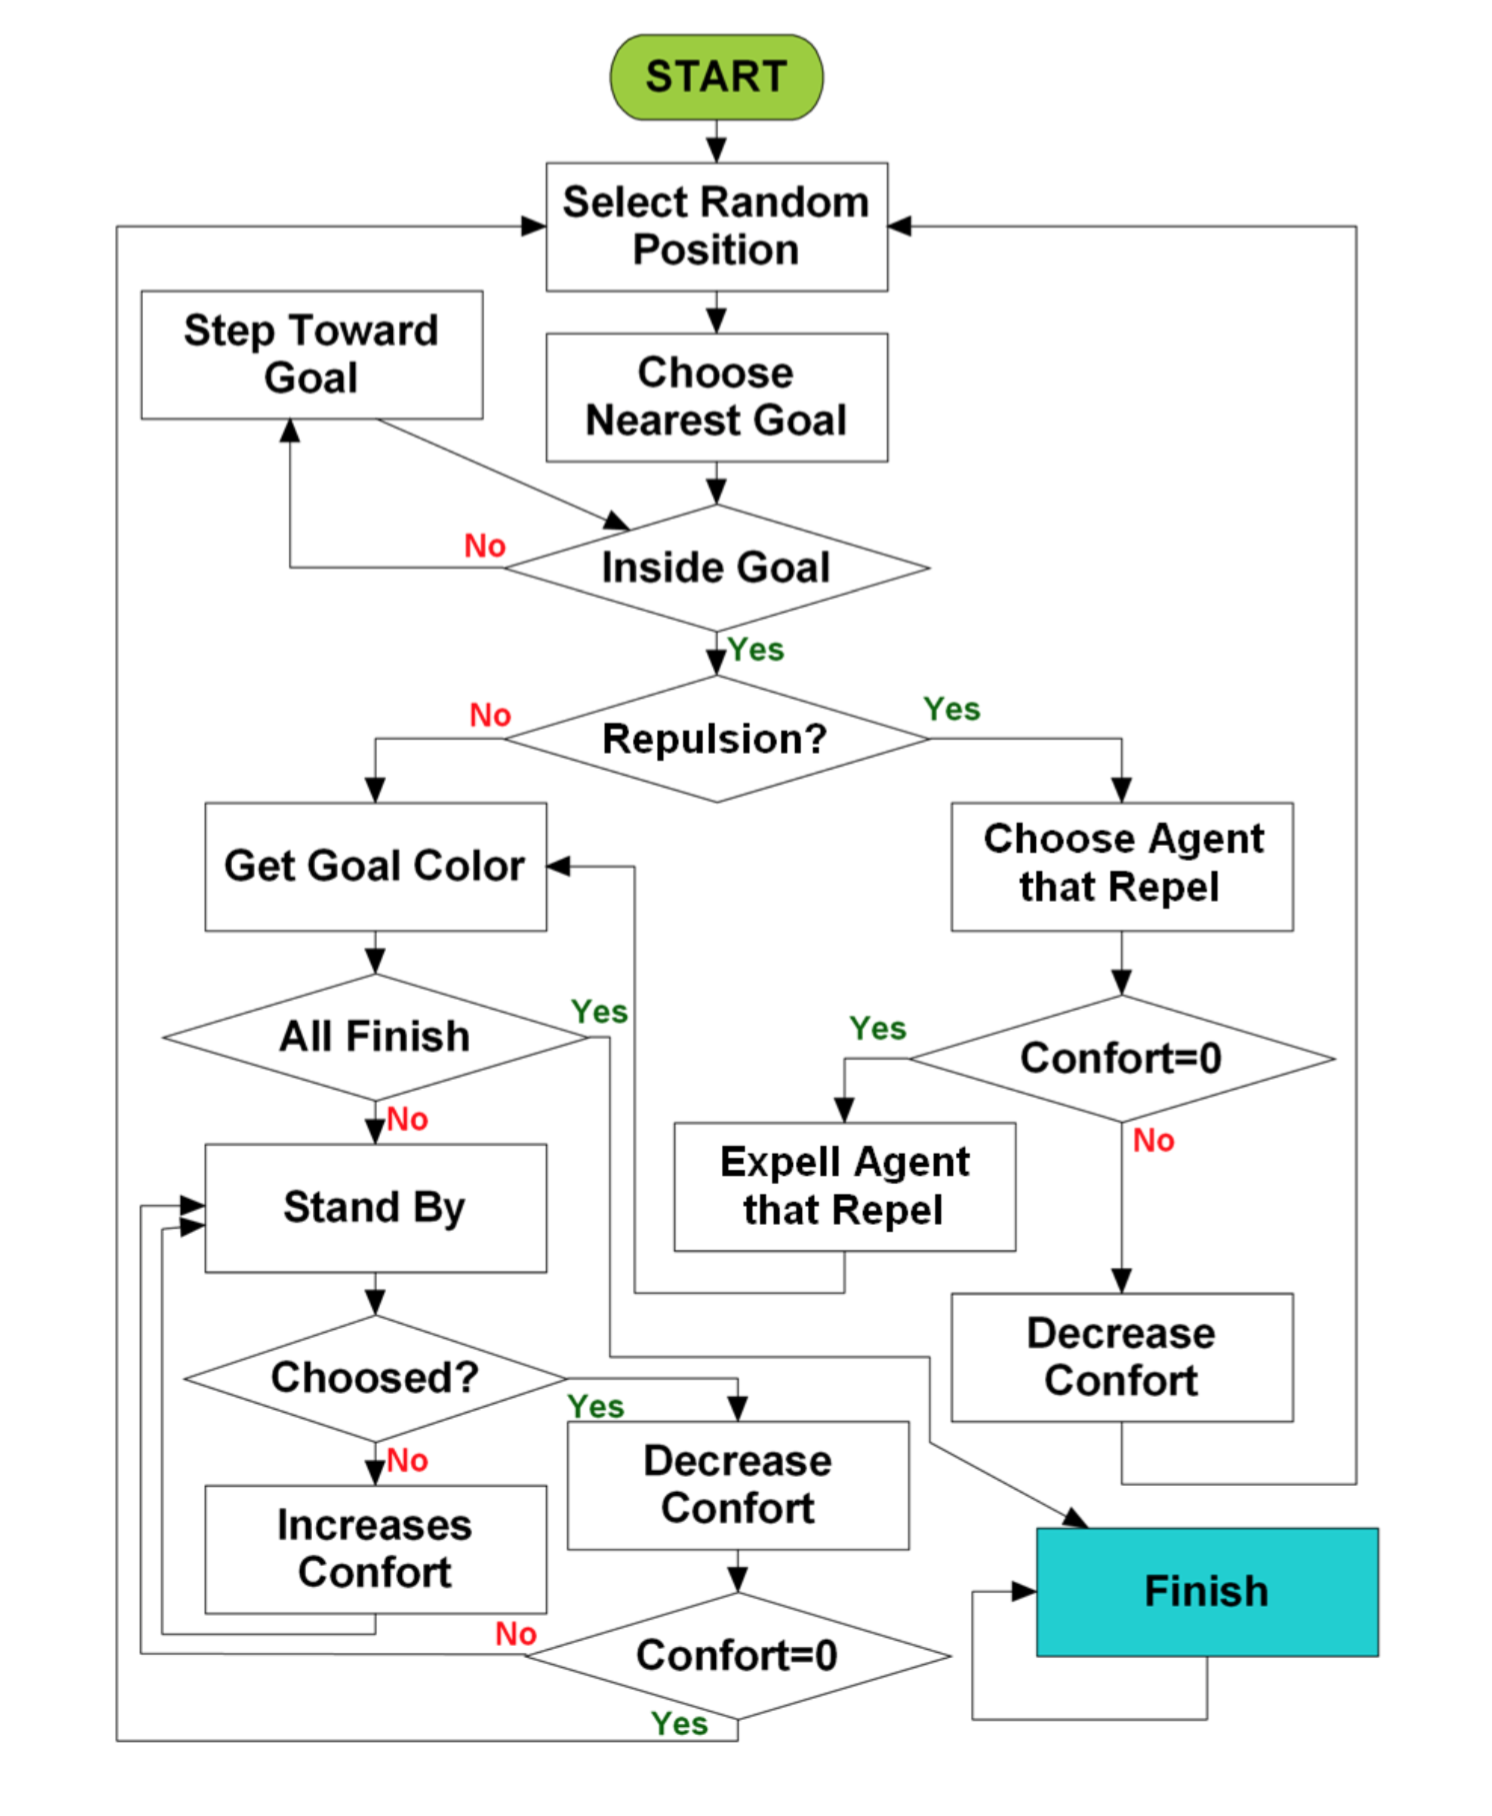
\includegraphics[scale=0.65]{gs-cp-flow}
\end{center}
Each agent moves in the toric world until all agents fall into the "Stand By" State. Then once the last agent triggers the "All Finished \Rightarrow Yes" State and the current colouring is accepted as valid. This algorithm presented some issues when implemented for testing. The comfort statistic that each agent tracks can grow unboundedly if the agents repeatedly fall into wells that they are repulsed from. This causes all agents to grow in comfort, making the local minuma deeper with every iteration and the chance of jumping out fall dramatically. 

\subsection{Workarounds}
\subsection{Additions}
\section{Genetic Algorithm}
The Genetic Algorithm presented here is a variant of the algorithm described by \cite{bib:GeneticAlg}. The algorithm was implemented as described, then tweaked to improve efficiency and to experiment with parameter tweaking and the effect of changing certain flows within the algorithm. These changes are discussed further in the Additions (\ref{genAdditions}) section. 

\subsection{Implementation and Problems}
The algorithm is implemented as follows:

\begin{algorithm}[H]
    \caption{Genetic Algorithm with Wisdom of Crowds}
    \label{alg:GA}
    \begin{algorithmic}[1] % The number tells where the line numbering should start
        \Procedure{solve}{Graph $g$, $iterationLimit$, $numChromosomes$} \Comment{$g$ is predefined}			
			\State $currentAttempt \gets 0$	
			\State $currentBestColouring \gets \Delta \left( g \right) +1$
			\State $aggregateChromosome \gets$ chromosome of randomly assigned colours.
			
			\While{$currentIteration < iterationLimit$}         
				\State $population \gets$ set of chromosomes with randomly assigned colours. (up to $numColours$)
				\If{solvePop()}
					\State $aggregateChromosome \gets$ chromosome of randomly assigned colours.
					\State $currentAttempt \gets 0$
				\Else
					\State $currentAttempt \gets currentAttempt + 1$
				\EndIf
         
            \EndWhile
            \State \textbf{return} $currentBestColouring$
        \EndProcedure
    \end{algorithmic}
\end{algorithm}

\begin{algorithm}[H]
\caption{Genetic Algorithm with Wisdom of Crowds - Tick Generation}
	\begin{algorithmic}[1]
    		\Procedure{solvePop}{Graph $g$, $iterationLimit$, $numChromosomes$} \Comment{$g$ is predefined}
    			\State $currentIteration \gets 0$
    			\While{$currentIteration < iterationLimit$ and best solution has cost $>$ 0}
    				\State $currentIteration \gets currentIteration + 1$
				\If{best chromosome has cost $\geq$ altMethodThreshold}			
    					\State $parents \gets getParentsA()$
    				\Else
    					\State $parents \gets getParentsB()$
    				\EndIf
    				\State $child \gets crossOver(parents)$
    				\If{rand $<$ mutChance}
    					\If{best chromosome has cost $\geq$ altMethodThreshold}
    						\State $child \gets mutateA()$
    					\Else
    						\State $child \gets mutateB()$
    					\EndIf
    				\EndIf
    				\State add $child$ to $population$
    				\State remove bottom performing half of population
    				\State repopulate up to numChromosomes
    			\EndWhile
    			\If{$currentIteration \geq iterationLimit$}
    				\State perform $wisdomOfCrowds()$ \Comment{generate $aggregateChromosome$ by voting}
    				\State add $aggregateChromosome$ to population
    			\EndIf
    			\If{best solution has cost 0}
    				\State $currentBestSolution \gets currentBestSolution -1$
    				\State \textbf{return} true
    			\Else
    				\State \textbf{return} false
    			\EndIf
   		\EndProcedure
    \end{algorithmic} 
\end{algorithm}

\begin{algorithm}[H]
\begin{algorithmic}[1]
\caption{Genetic Algorithm with Wisdom of Crowds - Parent Selection}
	\Procedure{getParentsA}{}
		\State $tempParents \gets$ choose two random chromosomes from population.
		\State $parent1 \gets$ fitter of $tempParents$
		\State $tempParents \gets$ choose two random chromosomes from population.
		\State $parent2 \gets$ fitter of $tempParents$
		\State \textbf{return} $parent1$, $parent2$
	\EndProcedure\\
	%\linebreak
	\setcounter{ALG@line}{0}
	\Procedure{getParentsB}{}
		\State \textbf{return} top performing chromosome, top performing chromosome
	\EndProcedure
\end{algorithmic}
\end{algorithm}

\begin{algorithm}
\begin{algorithmic}[1]
\caption{Genetic Algorithm with Wisdom of Crowds - Crossover}
	\Procedure{crossOver}{}
		\State $child \gets$ colours up to and including a random point from $parent1$, followed by the colours from $parent2$ from that point on in the chromosome.
		\State \textbf{return} child
	\EndProcedure
\end{algorithmic}
\end{algorithm}

\begin{algorithm}[H]
\begin{algorithmic}[1]
\caption{Genetic Algorithm with Wisdom of Crowds - Child Mutation}
	\Procedure{MutateA}{}
		\ForAll{$vertex$ in chromosome}
			\If{$vertex$ has a conflict}
			\State $adjacentColours \gets$ all adjacent colours to $vertex$
			\State $validColours \gets allColours - adjacentColours$
			\State $newColour \gets$ random colour from $validColours$
			\State set chromosome colour at $vertex$ to be $newColour$
			\EndIf
		\EndFor
	\EndProcedure\\
	%\linebreak
	\setcounter{ALG@line}{0}
	\Procedure{MutateB}{}
		\ForAll{$vertex$ in chromosome}
			\If{$vertex$ has a conflict}
				\State $newColour \gets$ random colour from allColours
				\State set chromosome colour at $vertex$ to be $newColour$
			\EndIf
		\EndFor
	\EndProcedure
\end{algorithmic}
\end{algorithm}

\begin{algorithm}[H]
\begin{algorithmic}[1]
\caption{Genetic Algorithm with Wisdom of Crowds - Wisdom Of Artificial Crowds}
	\Procedure{WisdomOfCrowds}{}
		\State $expertChromosomes \gets$ best half of final population
		\State $aggregateChromosome \gets$ best performing chromosome
		\ForAll{$vertex$}{$g$}
			\If{$vertex$ is part of a bad edge}
				\State $newColour \gets$ the most used colour for $vertex$ among $expertChromosomes$
				\State set colour at $vertex$ of $aggregateChromosome$ to be $newColour$
			\EndIf
		\EndFor
	\EndProcedure
\end{algorithmic}
\end{algorithm}

\subsection{Workarounds}
The algorithm provides some parameters to tailor the solving method to be able to deal with local optima in several ways. Firstly there are 2 different parent selection methods that are used depending upon how close the best chromosome is to a valid colouring. Secondly there are two different mutation methods that are used depending upon how close the best chromosome is to a valid colouring.
It was found that while these methods allowed for some level of control over the algorithm, it was by no means as configurable as the other algorithms that were implemented. To remedy this and to produce our own variant of the Genetic Algorithm for solving the GCP, alterations were made to the flow to allow more control over the algorithm.

\subsection{Additions}
\label{genAdditions}
The first deviation to the documented algorithm was to the parent selection criterion. It was found that having the best solution be the only parent that is mutated when it is sufficiently close to a valid colouring slowed the convergence rate of the other chromosomes to zero. To remedy this, we implemented a switch such that a certain percent of the time, the parents chosen were the best chromosome and itself. But a small percentage of the time, the parents would be the best chromosome and a random chromosome from the population. This prevented the stagnation of the problem, and allowed for other changes to be made to improve the algorithm. The second part of the algorithm identified for change was the crossover method. This method originally selected the first portion of $parent1$ and mixed it with the complement of that section of $parent2$. This process was changed to a simple 50/50, such that the chance of the first section coming from $parent1$ was equally weighted to the first section coming from $parent2$. This prevented possible bad colourings from being propagated simply because the occurred early in the chromosome. 
The final change to the algorithm was in response to results collected from the algorithm. It was found the wisdom of crowds voting mechanism was finding the solution far more successfully than the Genetic Algorithm itself. This prompted a change to the algorithm whereby a vote could not take place before certain conditions were met in the agreement of the chromosomes. This lead to a much higher runtime for the algorithm, but once a vote could commence, the algorithm was much more likely to either improve the colouring or produce a chromosome with many fewer conflicts. This method was settled upon after several other methods were trialed and discarded. As the algorithm searches for a tighter colouring, it takes many more generations for the chromosomes to converge. This method was settled upon since it allowed the algorithm to be applied to any graph with a minimum of tweaking, yet a valid vote will always take place, since the algorithm will always reach a point of agreement, even if the solution is not valid for the given graph. Setting the level of agreement that each chromosome must exhibit allows the algorithm to be sped up or slowed down. If the limit is relaxed, each trial takes less time to complete, yet the wisdom of crowds vote has a lower chance of improving the solution. Tightening the bounds has the effect of dramatically increasing the runtime of the algorithm but increases the chance that the wisdom of crowds vote will yield a better solution. Setting the bound too tight however will result in the algorithm running for an infinite amount of time (if the level of agreement specified is not possible).
The last change that was made to this algorithm was to create a variable parameter for how much of the population was discarded and repopulated at random  on each generation. This parameter is responsible for setting how much of the solution space is tried. Each iteration, the random nature of the generation process has the possibility to generate a better solution to the problem. However, the larger the proportion of the population that is discarded upon each iteration, the lower probability that the wisdom of crowds vote that occurs at the end of each trial will improve upon the solution. For this reason, the proportion of the population that is allowed to participate in the vote is set to always be less than (or equal to) the proportion that is kept in each iteration, so that random noise is not added to the voted data when a vote takes place.
\section{Flower Pollination}
\subsection{Implementation and Problems}

Ok so I have to say that I think that this paper\cite{7175923} SUCKS. I was drawn to it initially because it was a new (2015) optimisation algorithm and we wanted something to compare to the gravitational swarm intelligence\cite{bib:GravSwarm}, plus it was flowers which is cute.
Anyway, the first warning sign should have been that it's from Algeria, but that would have been racist. Second warning sign: THEY WORD FOR WORD COPIED from Yang's paper. Like, full blown plagiarism. Damn, how does that pass peer review??? Of course, I hadn't actually read Yang's paper at the start so I didn't know that.. Third warning sign: The algorithm doesn't quite match up with the pollination properties it supposedly takes inspiration from. Ok, not just these guys fault, Yang does the same thing.
So I tried to implement it. And I failed. Some parts of the pseudocode I just didn't know what they were talking about, and when I managed to work around that to hobble something together that ran, it just didn't do anything. So I hacked and hacked and made something that started to work! But it was still rubbish.

The original algorithm is as follows


\begin{algorithm}[H]
    \caption{FPA for GCP}
    \label{FPA1}
    \begin{algorithmic}[1] % The number tells where the line numbering should start
        \Procedure{solve}{Graph $g$, $iterationLimit$, $numFlowers$} \Comment{$g$ is predefined}			
			\State Initialize a population of $N$ flowers/pollen gametes with random solutions
			\State Find the best solution $g_*$ in the initial population
			\State Define a switch probability $p \in [0,1]$
			\State $t=0$
			\While{$t < iterationLimit$}   
				\For{$i=1:N$}
					\If{$rand < p$} \Comment{$rand$ is a function that returns a single uniformly distributed random number between 0 and 1}
						\State Draw a (d-dimensional) step vector $L$ which obeys a L\`evy distribution.
						\State Global pollination via $x_i^{t+1} = x_i^{t} + L(x_i^{t} - g_*)$
					\Else
						\State Draw $U$ from a uniform distribution $[0,1]$
						\State Do local pollination via $x_i^{t+1} = x_i^{t} + \epsilon(x_j^{t} - x_k^{t})$
					\EndIf
					\State //Discretisation and correction step
					\State Apply round function to obtain integer values
					\State Correction Step() \Comment{To ensure that no invalid colors are used.}
					\If{all $k$ colors are assigned}
						\State Swap the most conflicting node with a random vertex of the lowest used color
						\State Evaluate new solutions $x^{t+1}$ using global pollination
						\If{$f(x^{t+1})<f(x^{t})$}\Comment{If new solutions are better}
							\State $x^t = x^{t+1}$
						\EndIf
					\Else continue
					\EndIf
				\EndFor
				\State Update the current best solution $g_*$
					\If{$f^* == 0$}
					\Comment{Legal coloring found}
						\State $k = k-1$
						\State \textbf{Break}
					\EndIf
			\State $t = t+1$
			\EndWhile
			\State Output the best solution found
		\EndProcedure
    \end{algorithmic}
\end{algorithm}


The Correction Step() is also described, but it's so simple I'm not sure why they bothered. If a color class is assigned that is greater than $k$ instead set it to $k$, if a color class is assigned that is less than zero instead set it to zero.
Note that the \textbf{Break} when a legal coloring for a given $k$  is found should probably be a \textbf{Return} since it is implied (poorly) that this solve procedure exists within a larger framework for descending $k$.


\subsection{The Hacking}

Since the paper does such a poor job of describing the process, I was unable to implement the algorithm in such a way that it was capable of finding even a $k = \Delta$ coloring in an arbitrary \emph{reasonable} time (couple of hours). Frustrated, I made some rather drastic changes without much justification. I will now describe the final algorithm that \emph{sometimes} beats the genetic algorithm (see results).

First let's look at the algorithm

\begin{algorithm}[H]
    \caption{modified FPA for GCP}
    \label{FPA2}
    \begin{algorithmic}[1] % The number tells where the line numbering should start
        \Procedure{solve}{Graph $g$, $iterationLimit$, $numFlowers$} \Comment{$g$ is predefined}			
			\State Initialize the flowerbed
			\State Update the current best solution $g_*$
			\State Define a switch probability $p \in [0,1]$
			\State $t=0$
			\While{$t < iterationLimit$}   
				\For{$flowerNum = 0; flowerNum < numColours; flowerNum++$}
					\State fixColors(flowerNum)
					\If{$rand < p$} \Comment{$rand$ is a function that returns a single uniformly distributed random number between 0 and 1}
						\State Draw a (d-dimensional) step vector $L$ which obeys a L\`evy distribution.
						\State Global pollination via $x_i^{t+1} = x_i^{t} + L(x_i^{t} - g_*)$
					\Else
						\State Draw $U$ from a uniform distribution $[0,1]$
						\State Do local pollination via $x_i^{t+1} = x_i^{t} + \epsilon(x_j^{t} - x_k^{t})$
					\EndIf
					\State fixColors(flowerNum)
					\State Apply round function to obtain integer values
					\State Correction Step \Comment{To ensure that no invalid colors are used.}
					\For{$col = 0 : \alpha$} \Comment{$\alpha$ could be anything, currently set to $k$}
						\State swap(flowerNum)
					\EndFor
				\EndFor
				\State Update the current best solution $g_*$
				\If{$f^* == 0$}
					\State $k = k-1$
					\State \textbf{Return}
				\EndIf

				doNaturalSelection()
				\State $t = t+1$
			\EndWhile
			\State Output the best solution found
		\EndProcedure
    \end{algorithmic}
\end{algorithm}

Ok so as mentioned before, we call the set of flowers the \emph{flowerbed}. The main differences are as follows:

fixColors()
In the original algorithm, each flower is checked to see if every $k$ color is assigned. Only if that returns true is the swap strategy and global pollination perturbation performed. I found this to be odd, but rather than remove it I went the other direction and wrote a function that ensured that all colors are present. Simply put, fixColor searches the flower for each color in turn and if a color is not present it assigns that color to a random vertex.

fixColors is run before and after pollination to ensure that every flower adheres to the current $k$.

Rather than performing swap once, under the suspicion that swap is the main mover in the algorithm, I perform swap an arbitrary $\alpha$ number of times. For the purpose of experimentation, of which we report the results on later,  $\alpha = k$ without justification. Swap is directly reducing the cost and so moves the solution vector very quickly through the solution space towards a, presumably, local optima.

doNaturalSelection()
Despite regularly referring to, and comparing against, the genetic algorithm, the authors chose not to implement natural selection or wisdom of crowds. I didn't have the motivation to work out how wisdom of crowds would work for the flowerbed, however implementing natural selection was incredibly straightforward.
The cost of each flower in the flowerbed is assessed and the median value calculate. Every flower with a cost higher than the median value is replaced with a randomly generated flower.
Doing this is a response to the tending towards homogeneity that we've remarked upon before. Every iteration the available genetic material gets a massive shake-up, providing potentially new color partitions that might lead to a legal coloring.

That's pretty much it for flower pollination.











\chapter{Results \& Discussion}

\section{Algorithms}



\begin{table}[H]
\centering
\begin{tabular}{l l l l l l l l}
\hline
Graph & $\chi$ & $\Delta + 1$ & Solver & Limits on Runtime & k & time to k & \% success\\ \hline

queen5\_5.col & 5 & 17 & RBB & 100000 & 5 & time to k & percent\\
queen5\_5.col & 5 & 17 & GS & 1000000 & 5 & time to k & percent\\
queen5\_5.col & 5 & 17 & FPA & 10000 & 7 & time to k & percent\\
queen5\_5.col & 5 & 17 & GA & 20000 & 7 & time to k & percent\\

myciel5.col & 6 & 24 & RBB & 100000 & 3 & time to k & percent\\
myciel5.col & 6 & 24 & GS & 1000000 & 2 & time to k & percent\\
myciel5.col & 6 & 24 & FPA & 10000 & 10 & time to k & percent\\
myciel5.col & 6 & 24 & GA & 20000 & 8 & time to k & percent\\

queen7\_7.col & 7 & 25 & RBB & 100000 & 7 & time to k & percent\\
queen7\_7.col & 7 & 25 & GS & 1000000 & 9 & time to k & percent\\
queen7\_7.col & 7 & 25 & FPA & 10000 & 19 & time to k & percent\\
queen7\_7.col & 7 & 25 & GA & 20000 & - & - & percent\\

mulsol.i.3.col & 31 & 158 & RBB & 100000 & 31 & 2844 & percent\\
mulsol.i.3.col & 31 & 158 & GS & 1000000 & 31 & time to k & percent\\
mulsol.i.3.col & 31 & 158 & FPA & 10000 & - & - & percent\\
mulsol.i.3.col & 31 & 158 & GA & 20000 & - & - & percent\\

\hline
\end{tabular}
\caption{Results showing the time taken for the algorithm to find a valid colouring (k colours), optimal or not}
\label{res:timeToK}
\end{table}

\begin{table}[H]
\centering
\begin{tabular}{l l l l l l l l}
\hline
Graph & $\chi$ & $\Delta + 1$ & Solver & Limits on Runtime & min k reached & time to k & total runtime \\\hline
myciel4.col & 6 & 12 & RBB & 100000 & 3 & time to k & 470.3\\
myciel4.col & 6 & 12 & GS & 1000000 & 2 & time to k & $1.63 \times 10^7$\\
myciel4.col & 6 & 12 & FPA & 10000 & 10 & time to k & 4899871.0\\
myciel4.col & 6 & 12 & GA & 20000 & 8 & time to k & 2008825\\

queen5\_5.col & 5 & 17 & RBB & 100000 & 5 & time to k & 395.7\\
queen5\_5.col & 5 & 17 & GS & 1000000 & 5 & time to k & 1382389\\
queen5\_5.col & 5 & 17 & FPA & 10000 & 7 & time to k & 2136729\\
queen5\_5.col & 5 & 17 & GA & 20000 & 7 & time to k & 7211935\\

myciel5.col & 6 & 24 & RBB & 100000 & 3 & time to k & 470.3\\
myciel5.col & 6 & 24 & GS & 1000000 & 2 & time to k & $1.63 \times 10^7$\\
myciel5.col & 6 & 24 & FPA & 10000 & 10 & time to k & 4899871.0\\
myciel5.col & 6 & 24 & GA & 20000 & 8 & time to k & 2008825\\

queen7\_7.col & 7 & 25 & RBB & 100000 & 7 & time to k & 780.0\\
queen7\_7.col & 7 & 25 & GS & 1000000 & 9 & time to k & $1.23 \times 10^7$\\
queen7\_7.col & 7 & 25 & FPA & 10000 & 19 & time to k & 13875131\\
queen7\_7.col & 7 & 25 & GA & 20000 & - & - & -\\

mulsol.i.3.col & 31 & 158 & RBB & 100000 & 31 & 2844 & 4952\\
mulsol.i.3.col & 31 & 158 & GS & 1000000 & 31 & time to k & 21604849\\
mulsol.i.3.col & 31 & 158 & FPA & 10000 & - & - & -\\
mulsol.i.3.col & 31 & 158 & GA & 20000 & - & - & -\\

\hline
\end{tabular}
\caption{Results of algorithms attempts at finding a better solution (and failing)}
\label{res:timeToFail}
\end{table}
\chapter{Bibliography}
\begin{thebibliography}{}

\bibitem{bib:GravSwarm}
Israel Carlos Rebollo Ruiz. 
\textit{Gravitational Swarm for Graph Coloring}. 
http://www.ehu.eus/ccwintco/uploads/3/3a/Tesis-Israel-final.pdf, 2012.

\end{thebibliography}

\end{document}